\documentclass{article}
\usepackage{fullpage}
\usepackage{amsmath,amssymb,amsfonts}
\usepackage{graphicx}
\usepackage{natbib}

\def\R{{\mathbb{R}}}
\def\pr{{\rm Pr}}
\def\E{{\mathbb E}}
\def\X{{\mathcal X}}
\def\Y{{\mathcal Y}}
\def\H{{\mathcal H}}
\def\G{{\mathcal G}}
\def\B{{\mathcal B}}
\def\yh{{\widehat{y}}}
\def\bias{{\rm bias}}
\def\supp{{\rm supp}}
\def\dist{{\rm dist}}
\def\sign{{\rm sign}}
\def\vol{{\rm vol}}
\def\PL{{\mbox{\rm PL}}}

\newtheorem{thm}{Theorem}
\newtheorem{lemma}[thm]{Lemma}
\newtheorem{cor}[thm]{Corollary}
\newtheorem{claim}[thm]{Claim}
\newtheorem{defn}[thm]{Definition}
\newtheorem{assump}{Assumption}
\newtheorem{open}{Open problem}
\newenvironment{proof}{\noindent {\sc Proof:}}{$\Box$ \medskip}

\newcommand{\comment}[2]{ {\bf #1 :} #2}
\newcommand{\yoav}[1]{\comment{Yoav}{#1}}
\newcommand{\sanjoy}[1]{\comment{blue}{Sanjoy}{#1}}

\DeclareMathOperator*{\argmax}{arg\,max}

\title{Active learning using region-based sampling}

\begin{document}

\maketitle

\section{Introduction}

In active learning, labels of individual points are not available immediately but can be obtained for a price. The goal is to find a good model, or to label a data set, at low cost.

We consider a formulation in which we have a collection of $n$ points $X = \{x_1, \ldots, x_n\}$ that lie in a metric space $(\X, d)$. We can request the label of any of these points $x$, in which case we get a value $y \in \{-1, +1\}$ with unknown conditional distribution
$$ \eta(x) = \E[y | x] = \pr(y=1|x) - \pr(y=-1|x) = 2 \pr(y=1|x) - 1 .$$
The \emph{Bayes-optimal} label for $x$ is then 
$$ g^*(x) = \left\{
\begin{array}{cl}
-1 & \mbox{if $\eta(x) < 0$} \\
+1 & \mbox{if $\eta(x) > 0$} \\
\mbox{either} & \mbox{if $\eta(x)= 0$}
\end{array} \right.
$$
We wish to find the Bayes-optimal labels for $X$.

More precisely, at the outset we have only the finite data set $X$, and are also given parameters $0 < \gamma, \delta < 1$ and the number of queries the algorithm is allowed to make, called the query budget. We want a procedure that chooses the next point, or batch of points, to query. This process will be applied repeatedly until the query budget is exhausted, whereupon labels $\yh(x)$ must be provided for all $x \in X$, including those that were queried. Ideally, these will equal the Bayes-optimal labels $g^*(x)$, but we will only be judged on points $x \in X$ with $|\eta(x)| \geq \gamma$. That is, the number of mistakes is taken to be:
$$ \sum_{x \in X} {\bf 1}(\yh(x) \neq g^*(x),\ |\eta(x)| \geq \gamma) .$$
The overall procedure is allowed to fail with probability $\delta$, to account for sampling error.

\iffalse
\yoav{I think the discussion of sampling once vs sampling multiple times is too in the weeds for the introduction}
In some applications, a point $x$ can be queried repeatedly, with each resulting label being an independent draw according to $\eta(x)$. If this is the case, it is enough to query each point $O(1/\gamma^2)$ times and take the majority label, giving a total label complexity of $O(n/\gamma^2)$. For maximum generality, we do not assume that \emph{repeat querying} is allowed and thus we query each point at most once. If repeat queries are permissible, $O(1/\gamma^2)$ copies should be made of each point in $X$ before our method is applied.
\footnotesize
\fi

\subsection{Nonparametric active learning}

In our setting there is no underlying assumption about $g^*$, for
instance that it follows a linear model. Thus we adopt a nonparametric
approach.

There are several existing proposals for nonparametric active
learning, including those of
\citep{CN08,DH08,M12,DNZ15,H17,ASU18}. These algorithms can be
partitioned according to the overall principle they follow: either (1)
they seek to obtain the Bayes-optimal labels of a few well-positioned
points, and then propagate these to the rest of the space
\cite{DNZ15,H17,ASU18} or (2) they estimate the biases (positive or
negative) of entire regions at a time \cite{DH08,M12}. In this paper,
we follow the second strategy because the only reliable and
general-purpose way to assess the sign---that is,
$\mbox{sign}(\eta(x))$---of an individual point is to query that
particular point repeatedly: absent smoothness assumptions, the sign
can change abruptly in an arbitrarily small neighborhood around
$x$. On the other hand, determining if $\eta(B)>\gamma$ or if $\eta(B)<-\gamma$
requires a constant number of queries, independent of the size of $B$.

\subsection{Overlapping regions}

The overall active learning strategy is to use a set of regions of
different sizes $\B$ and to use label queries to estimate the sign (of
the bias) associated selected subsets of regions. A typical point
$x \in X$ is contained in many regions, we call the set of regions of
size $\ell$ that contain $x$ the $\ell$-{\em neighborhood} of $x$ and
denote it by $\B_\ell(x)$. Special significance is given to points $x$
where the set $\B_\ell(x)$ contains regions with opposing signs we
call these points ``known-unknowns'' or ``conflicts''. Conflict points
appear close to the classification boundary and are used to define the
regions for active sampling. Non-conflice points are provisionally
labeled according to the concensus sign of the neighborhood.

This design differs from earlier work on region based
non-parametric active learning~\cite{DH08,M12} where the regions form
a hierarchical partitioning of the space, so that each point is
covered by exactly region at each level.  For instance, \cite{M12}
uses a dyadic partitioning of the space at multiple levels of
granularity. This eliminates conflicts and thereby
requires different approach to drive active learning.

% We also adopt a hierarchical approach in the sense that
% we segregate the regions $\B$ according to size. We begin by
% estimating the sign of the largest of them, and then move on to
% progressively smaller neighborhoods as the need arises.

\subsection{Three key Challanges}
In giving shape to the proposed scheme, three key challenges need to to be addressed.

The first challenge is deciding \emph{where to query}. Suppose that a
particular region $B \subset \X$ has an average $\eta$-value close to
zero. Earlier work (e.g. \cite{DH08}) has taken this as a sign that
$B$ is part of the ``uncertainty'' region and should be queried
further. But it is important to distinguish two cases: (1) the $\eta$
values are close to zero throughout $B$, and (2) $B$ consists of two
sub-regions, one of which is strongly positive while the other is
strongly negative. In the first case, there is little merit in
querying further. But in the second case, there is a lot to be gained.

To distinguish these two cases, we use a collection of neighborhoods
that are \emph{overlapping}. For instance, we might take $\B$ to be
\emph{all} balls in $\X$, although this becomes a finite collection
once the given data points $X$ are taken into account. Case (2) can
then be detected: we think of a point $x$ as being in the uncertainty
region if it is contained in a region $B$ that is strongly
positive as well as being in a region $B'$ that is strongly
negative. Such points are ``known unknowns'', and these are the
targets of our active querying.

A second challenge is that even when a neighborhood $\B_\ell(x)$ has a
consistent sign, and thus a provisional label, it is possible that
$\B_{\ell+1}(x)$ has the opposite consistent sign resulting in a flipped provisional label.
Thus, if we consider 
successively smaller neighborhoods containing $x$, say
$\B_1(x) \supset \B_2(x) \supset \B_3(x) \supset \B_4(x) \cdots$, the provisional label for $x$
can keep changing.

% So at first, when we are querying regions of
% roughly the size of $B_1$, we might think $x$ has label $+1$. When we
% move to of the size of $B_2$, this could change to $-1$. And then back
% to $+1$, and son. We call these \emph{mind changes}.

In other words, at no point can we ever we sure that we have
correctly determined the label of $x$. Thus in addition to focused
(active) querying, we also do background sampling, of the entire
space, to pick up on regions where there might be mind changes. For
simplicity, we make one background query for each focused query.

The third challenge is \emph{managing sampling} when the neighborhoods
$\B$ are overlapping. Recall that we are interested in detecting
points, and thus neighborhoods, whose $\eta$-values are either
$> \gamma$ or $<-\gamma$. Thus suggests querying
$k \approx 1/\gamma^2$ points at random from each region. Now, suppose
we have queried this many points from neighborhood $B$ and then later
want to query points from a different neighborhood $B'$ that overlaps
$B$. How can we do this in a way that reuses the queries we have
already made in $B \cap B'$?

\emph{Poisson sampling} provides a clean solution. Rather than
choosing $k$ points at random from $B$, we pick each point in $B$ with
probability (roughly) $k/|B \cap X|$, independently. The specific way
we implement this is to assign each $x \in X$ a uniform-random value
$T_x \in [0,1]$, at the outset. When sampling $B$, we choose to query
$x$ if $T_x \leq k/|B \cap X|$. And when it comes time to sample a
different $B'$ that also contains $x$, we again choose $x$ if
$T_x \leq k/|B' \cap X|$; if its label has already been obtained, we
are able to reuse it. In this way, the random querying of overlapping
regions is seamlessly managed.

These three challenges go beyond earlier work in active learning,
which was able to avoid problems like mind-changes by making
smoothness assumptions on $\eta$. We propose a general-purpose active
learning scheme and are thus forced to deal with these issues.

Our algorithm does not require any assumption on the input
distribution. In the worst case the number of queries is twice the
number of queries of a passive algorithm. We show that under several
natural conditions the query complexity of our algorithm is
logarithmic in the error.

\subsection{Related work}

There is a small body of work on the theory of nonparametric active learning. The early results of \cite{CN08} established upper and lower bounds on label complexity in situations where the Bayes-optimal boundary is of a simple form: a single threshold for one-dimensional data or a ``smooth boundary fragment'' in higher dimension.

An algorithm for active learning based on hierarchical sampling was given in \cite{DH08} and was analyzed under smoothness conditions in \cite{KUB15}. In these works, the idea is to begin with a hierarchical clustering of $X$, and to then use queries to discover a pruning of this tree whose leaf-clusters are almost-pure in their labels. The method is not well-suited to situations with significant noise levels. Another approach using hierarchical dyadic partitions was given in \cite{M12} and analyzed under the commonly-used smoothness, margin, and density assumptions---namely, that $\eta$ is Holder-smooth, the fraction of points with $|\eta(x)| \leq t$ is some polynomial in $t$, and the marginal density is close to uniform---along with a more unusual smoothness requirement on $\eta$.

A different strategy using nearest neighbors was explored by \cite{ASU18}. Their idea was to choose an appropriate scale $s$, find an $s$-cover of $X$, estimate the Bayes-optimal label for each point in this cover by querying its neighbors, and then use these cleanly-labeled points for 1-nearest neighbor classification. A somewhat more general approach was given in \cite{H17} and studied under the usual smoothness, margin, and density conditions, with resulting rates of convergence comparable to those found by \cite{M12}.

Finally, \cite{DNZ15} suggested a graph-based method for active learning based on adaptively looking for the cut in the graph corresponding to the correct decision boundary. Their assumptions are based on properties of this graph cut and are thus not easy to directly relate to earlier work.


\section{The active learning algorithm}

\subsection{A collection of sampling regions}

In the active learning algorithm, sampling is organized around a
collection $\B$ of regions that are subsets of $\X$. These are the
atomic sets on which we assess label bias. While our general results
hold for arbitrary regions, there seems to be little cost to
restricting regions to be balls in our metric space. From here on out,
we will use the term ball instead of region.

For any ball $B \in \B$, let $X_B = X \cap B$ be a shorthand for the
data points that lie in it.\footnote{Since we use $X_B$ to assess the
  label bias of $B$, we will need to exclude points that cannot be
  considered random samples from $B$. For instance, consider these two
  alternatives: (1) $\B$ consists of a pre-defined set of balls. (2)
  $\B$ consists of balls defined by pairs of points in $X$, with each
  $x,x' \in X$ yielding the ball $B(x,\|x-x'\|)$. In the first case,
  all points $X \cap B$ are random draws from $B$. In the second case,
  we would need to exclude the two points $x,x'$ that define the
  ball.}

We group balls into levels by their size, which is the number of
points they contain. The ball $B$ is placed at {\it level}
$\ell \geq 0$ if
\begin{equation}
\frac{n}{2^{\ell + 1}} \leq |X_B| < \frac{n}{2^\ell} .
\label{eq:sampling-level}
\end{equation}
Let $\B_\ell$ consist of all balls in $\B$ that are at level $\ell$. Thus $\B_0, \B_1, \ldots$ is a partition of $\B$, with $\B_0$ consisting of very large balls and subsequent $\B_1, \B_2, \ldots$ consisting of successively smaller balls. We will use $\B_{\geq \ell}$ to denote all balls at levels $\ell$ or greater, and likewise $\B_{> \ell}$, $\B_{\leq \ell}$, and so on. 

Balls in lower levels are contain more points, and are, in a sense "easier". 
Our algorithm iterates over levels $\ell=1,2,3,\ldots$, making it's way from easier to harder levels.

For any $x \in \X$, let $\B(x) \subset \B$ denote the collection of balls that contain $x$ and can thus be used in determining $x$'s label. As before, we partition these balls by sampling-level, so that $\B_\ell(x) = \B(x) \cap \B_\ell$. We will also refer to $\B_\ell(x)$ as the {\em level $\ell$ neighborhood of $x$}

\subsection{Estimating bias}

We use label-queries to estimate the biases of balls $B \in \B$. 
These are in turn used to estimate the labels of individual points.

The bias of a ball $B \in \B$ is defined as
$$ \eta_X(B) = \mbox{average}\{\eta(x): x \in X_B \} .$$

Rather than working with a precise numerical estimate, we assign each ball a \emph{qualitative} bias estimate,
$$ \yh(B) = 
\left\{
\begin{array}{cl}
+1 & \mbox{significant $+$ bias} \\
-1 & \mbox{significant $-$ bias} \\
0 & \mbox{no significant bias} \\
\bot & \mbox{not yet available}
\end{array}
\right.
$$

The option $\bot$ is used until sufficiently many points in $X_B$ have been queried: the required number is $O(1/\gamma^2)$, recalling that $\gamma$ is the smallest bias that needs to be detected. Once this many labels are available, $\yh(B)$ is set to a value in $\{-1,0,+1\}$ and remains fixed thereafter. These bias estimates will with high probability be seen to satisfy the following guarantee.
\begin{defn}
For any $B \in \B$, we say bias estimate $\yh(B) \in \{+1,-1,0\}$ is \emph{$\gamma$-accurate} if the following holds:
\begin{itemize}
\item $\yh(B) = +1 \implies \eta_X(B) > 0$
\item $\yh(B) = -1 \implies \eta_X(B) < 0$
\item $\yh(B) = 0 \implies |\eta_X(B)| < \gamma$
\end{itemize}
\label{def:accurate-bias-estimate}
\end{defn}

Pick any point $x$ and any level $\ell$. Once qualitative bias estimates are available for all balls $B \in \B_\ell(x)$, the set of possible labels for $x$ at level $\ell$, denoted $\PL_\ell(x) \subset \{-1,+1\}$, is defined as follows:
\begin{itemize}
\item $\PL_\ell(x)$ contains $+1$ if there exists a \emph{minimal} ball $B \in \B_{\leq \ell}(x)$ (that is, which has no other $B' \in \B_{\leq \ell}(x)$ strictly contained with it) with $\yh(B) = +1$.
\item $\PL_\ell(x)$ contains $-1$ under a symmetrical condition.
\end{itemize}
This is spelled out precisely in Equation~(\ref{eq:PL}) in  in Figure~\ref{alg:main}. The label-estimate for $x$ at level $\ell$, denoted $\yh_\ell(x) \in \{+1,-1,0,!\}$, is computed based on $\PL_\ell(x)$ as defined in Equation~(\ref{eq:provisional-label}). The intepretation of $\yh_\ell(x) \in \{+1,-1,0\}$ is given in Equation~\ref{def:accurate-bias-estimate}. The label "!" can be interpreted as "known unknown"~\cite{Rumsfled}
or as "conflicting evidence". Our active learning algorithm makes "focused" queries in balls that contain known unknowns in order to resolve the label.

% to be $-1$ if $\PL_\ell(x) = %\{-1\}$, or $+1$ if $\PL_\ell(x) = \{+1\}$, or $0$ if $\PL_\ell(x) = \{\}$, or $!$ %if $\PL_\ell(x) = \{-1,+1\}$, %and remains fixed thereafter. Points labeled $!$ are ``known unknowns'': they are %near the decision boundary and %need further investigation. Points labeled $0$ show no significant bias.

\subsection{The neighborhoods active learning algorithm}

Our active learning algorithm is described in
Figures~\ref{alg:main},\ref{alg:sampling}.  A rough description of the
algorithm follows. There are two types of queries: focused queries and
background queries. The background queries correspond to passive
learning. Focused queries are made in the focus set $U_\ell$ and
correspond to active learning. The uncertainty region $U_\ell$ is the
union of all balls in $\B_{\ell}$ that contain a point on which the
prediction is "known unknown", $\yh_\ell(x)=!$.


% At each level $\ell$
% and each point $a$, the algorithm considers the Roughly speaking, the
% algorithm iterates over the levels $\ell=0,1,2,3,\ldots$, at each
% level and~\ref{alg:bias-estimate}. Central variables are the
% uncertainty regions $U_\ell$ which are all

\begin{figure}[h!]
\framebox{
\begin{minipage}[t]{6.4in}
\begin{itemize}
\item Initialize uncertainty regions at all levels:
\begin{itemize}
\item $U_0 = X$
\item $U_\ell = \emptyset$ for $\ell \geq 1$
\end{itemize}
\item Initialize labels at all levels to ``unavailable'':
\begin{itemize}
\item $\yh_\ell(x) = \bot$ for all $x$ and $\ell \geq 0$
\end{itemize}
\item Repeat:
\begin{itemize}
\item If there is a level $\ell \geq 0$ such that $U_\ell \neq \emptyset$:
\begin{itemize}
\item Let $\ell'$ be the smallest such level
\item {\tt Focused-query}($\ell', U_{\ell'}$)
\end{itemize}
\item {\tt Background-query}
\item Update labels:
\begin{itemize}
\item Update bias-estimates $\yh(B)$ as in Figure~\ref{alg:bias-estimate}
\item For each $x \in X$ and level $\ell \geq 0$ for which all $\{\yh(B): B \in \B_\ell(x)\}$ are available:
\begin{itemize}
\item Determine the possible labels for $x$ at level $\ell$:
\begin{equation} 
\begin{split}
\PL_\ell(x) = \{s \in \{-1, +1\}:\  & \mbox{there exists $B \in \B_{\leq \ell}(x)$ with $\yh(B) = s$} \\ 
& \mbox{and no other $B' \in \B_{\leq \ell}(x)$ has $X_{B'} \subsetneq X_B$.} \} 
\end{split}
\label{eq:PL}
\end{equation}
\item Set
\begin{equation} 
\yh_\ell(x) = 
\left\{
\begin{array}{cl}
+1 & \mbox{if $\PL_\ell(x) = \{+1\}$} \\
-1 &  \mbox{if $\PL_\ell(x) = \{-1\}$} \\
0 & \mbox{if $\PL_\ell(x) = \{\}$} \\
! & \mbox{if $\PL_\ell(x) = \{-1,+1\}$}
\end{array}
\right.
\label{eq:provisional-label}
\end{equation}
\end{itemize}
\end{itemize}
\item Update uncertainty regions:
\begin{itemize}
\item $U_0 = \{x \in X: \yh_0(x) = \bot\}$
\item For all levels $\ell \geq 1$: $U_\ell = \{x \in X: \yh_{\ell-1}(x) = \,!, \ \yh_\ell(x) = \bot\}$
\end{itemize}
\end{itemize}

\end{itemize}

\end{minipage}}
\caption{The active learning algorithm. Each iteration of the main loop makes (at most) one focused query and one background query. The subroutines {\tt Focused-query} and {\tt Background-query} appear in Figure~\ref{alg:sampling}.}
\label{alg:main}
\end{figure}

The querying process can be stopped at any time, whereupon labels are assigned as follows:
\begin{equation}
\yh(x) = 
\left\{
\begin{array}{ll}
\yh_\ell(x) & \mbox{for the largest $\ell$ with $\yh_\ell(x) \in \{-1,+1\}$, if such an $\ell$ exists} \\
0 & \mbox{(meaning ``don't know''), otherwise}
\end{array}
\right.
\label{eq:final-label}
\end{equation}

\begin{figure}[h!]
\framebox{
\begin{minipage}[t]{6.4in}

\vspace{.1in}
\emph{Initialization:}
\begin{itemize}
\item Set $Q = \emptyset$ (points queried so far)
\item For each $x \in X$: choose $T_x \sim \mbox{uniform}([0,1])$
\end{itemize}

\vspace{.2in}
{\bf Focused-query}($\ell, U$)

\vspace{.1in}
\begin{itemize}
\item Define querying region:
$$ S =  \bigcup_{x \in U} \bigcup_{B \in \B_\ell(x)} \{z \in X_B: T_z \leq \tau_\ell\} $$
\item Query the next unlabeled point in $S \setminus Q$, ordered by $T_z$ values, and add to $Q$
\end{itemize}

\vspace{.2in}
{\bf Background-query}

\vspace{.1in}
\begin{itemize}
\item Query the next unlabeled point in $X \setminus Q$, ordered by $T_z$ values, and add to $Q$
\end{itemize}
\end{minipage}}
\caption{The two sampling procedures. Each point $x \in X$ has an associated value $T_x$ chosen uniformly at random from $[0,1]$. This smaller this value, the earlier this point is likely to be queried. The focused querying procedure uses level-based thresholds $\tau_\ell = \min(2^{\ell+2}k/n, 1)$, where $k$ is a global parameter.} 
\label{alg:sampling}
\end{figure}


\begin{figure}[h!]
\framebox{
\begin{minipage}[t]{6.4in}
\vspace{.1in}
\begin{itemize}
\item Suppose $B \in \B_\ell$
\item Until all the points in $\{z \in X_B: T_z \leq \tau_\ell\}$ have been queried: define $\yh(B) = \bot$
\item Thereafter: let $\widehat{\eta}(B)$ be the mean of these labels and define
$$ \yh(B)
= 
\left\{
\begin{array}{ll}
\sign(\widehat{\eta}(B)) & \mbox{if $|\widehat{\eta}(B)| \geq \gamma/2$} \\
0 & \mbox{otherwise}
\end{array}
\right.
$$
\end{itemize}
\end{minipage}}
\caption{The qualitative bias $\yh(B)$ of a ball $B$.}
\label{alg:bias-estimate}
\end{figure}


\section{Analysis of algorithm: finite population setting}

We now analyze the active learning procedure in a setting where $X \subset \X$ is an arbitrary set of $n$ points; that is, we make no distributional assumption on the manner in which $X$ is generated.

\subsection{Accuracy of bias estimates}

Fix the set of balls $\B$. We start with a uniform guarantee on the
bias estimates for all balls $B \in \B$.  Let $0 < \delta < 1$ to be a
predefined confidence parameter, and define the constants $c,k$ as
follows:
\begin{equation}
c = \sqrt{3 \ln \frac{4|\B|}{\delta}} .
\label{eq:c1}
\end{equation}
and
\begin{equation}
  k =  \lceil (8c/\gamma)^2\rceil
\end{equation}
This choice of $k$ is determined by the following result, proved in the appendix.
\begin{lemma}
Suppose that $k \geq (8c/\gamma)^2$ where $c$ is given in (\ref{eq:c1}). 
For each $B \in \B$, let $\yh(B)$ be defined as in Figure~\ref{alg:bias-estimate}. Then with probability $\geq 1-\delta$, all the $\yh(B)$, for $B \in \B$, are $\gamma$-accurate.
\label{lemma:accurate-bias-estimates}
\end{lemma}

In what follows, we will assume that for all  $B \in \B$, $\yh(B)$ is $\gamma$-accurate.


\subsection{Critical levels}

The label assigned to a data point $x$ at level $\ell$, which we denote $\yh_\ell(x)$, might change as $\ell$ increases; it may flip between $+1$ and $-1$ a few times, with stretches of $0$ or $!$ in between. This $\yh_\ell(x)$ is governed by $\PL_\ell(x) \subset \{-1,+1\}$, the ``possible labels'' for $x$ given the information from balls at levels $0$ through $\ell$. 

The quantities $\yh_\ell(x)$ and $\PL_\ell(x)$ depend upon the random choices of the querying algorithm and might not allow

Nevertheless, it is possible to define two critical levels for each $x$: a level $L_1(x)$ by which $\PL_\ell(x)$ will reliably contain the correct label of $x$, and a level $L_2(x)$ by which $\PL_\ell(x)$ will reliably omit the wrong label.

\begin{defn}
Pick any $x \in X$ with $\eta(x) \neq 0$ and let $s(x) = \sign(\eta(x))$ be its Bayes-optimal label. We define $L_1(x)$ to be the smallest level $\ell$ such that:
\begin{itemize}
\item There exists some $B_o \in \B_\ell(x)$ with $s(x) \cdot \eta_X(B_o) \geq \gamma$.
\item Any $B \in \B(x)$ with $X_{B} \subset X_{B_o}$ also has $s(x) \cdot \eta_X(B) \geq \gamma$.
\end{itemize}
We define $L_2(x)$ to be the smallest level $\ell$ such that:
\begin{itemize}
\item For all $B \in \B_{\geq \ell}(x)$, we have $s(x) \cdot \eta_X(B) \geq 0$.
\item For any $B \in \B_{\leq \ell}(x)$ with $s(x) \cdot \eta_X(B) < 0$, there exists $B' \in \B_{\leq \ell}(x)$ with $X_{B'} \subset X_B$ and $s(x) \cdot \eta_X(B') \geq 0$.
\end{itemize}
Take $L_1(x)$ or $L_2(x)$ to be $\infty$ if no level meets the requirements. 
\label{defn:L12}
\end{defn}

The significance of these definitions is made clear by the following lemma, proved in the appendix.

\begin{lemma}
Pick any $x \in X$ with $\eta(x) \neq 0$ and let $s(x) \in \{+1,-1\}$ denote its Bayes-optimal label. Then for any level $\ell$ and any time at which $\yh_\ell(x) \neq \bot$:
\begin{enumerate}
\item[(a)] If $\ell \geq L_1(x)$, then $s(x) \in \PL_\ell(x)$ and thus $\yh_\ell(x) \in \{s(x), !\}$. 
\item[(b)] If $\ell \geq L_2(x)$, then $-s(x) \not\in \PL_\ell(x)$ and thus $\yh_\ell(x) \in \{s(x), 0\}$.
\end{enumerate}
\label{lemma:boundary}
\end{lemma}

\subsection{Boundary sets and label complexity}

A common intuition regarding active learning is that the label of
instances far from th decision boundary can be determined after fewer
queries than those that are close to the boundary. We follow this
intuition to define aboundary sets.

Fix a point $x$ As the level $\ell$ increases, the algorithm considers
smaller balls $\B_\ell(x)$. Intuitively, if $x$ is far from the
decision boundary, then for a sufficiently large $\ell$, $\yh(B)$ has
the same sign for $\forall B \in \B_\ell(x)$ and we do not need to
query the label of $x$. Based on this intuition we define the boundary

\begin{defn}
For any level $\ell$, define the \emph{boundary set} at level $\ell$ to be
\begin{equation}
\Delta_\ell 
= \bigcup_{x \in X: L_2(x) \geq \ell} \bigcup_{B \in \B_{\ell}(x)} X_B 
.
\label{eq:sampling-region}
\end{equation}
\end{defn}

It can be shown that all focused samples at level $\ell$ will lie in this set.
\begin{lemma}
All focused samples at level $\ell$ lie in $\{z \in \Delta_\ell: T_z \leq \tau_\ell \}$.
\label{lemma:focused}
\end{lemma}

We can now give generic label complexity bounds in terms of the quantities $L_1$, $L_2$, and $\Delta_\ell$.


\begin{thm}
Suppose the active learning algorithm makes $0 < m \leq n$ queries. Then all points $x \in X$ with $L_1(x) \leq \ell_1$ and $L_2(x) \leq \ell_2$ will get correct labels $\yh(x) = g^*(x)$, where
$$ \ell_1 = \left\lfloor \lg \frac{m}{32k} \right\rfloor $$
and $\ell_2$ is the largest integer $\leq \lg (n/2k)$ such that
$$ \sum_{\ell = \ell_1 + 1}^{\ell_2} |\Delta_{\ell}| \, 2^{\ell+2} \ \leq \ \frac{mn}{8k} .$$
\label{thm:label-complexity}
\end{thm}

A more local form of this result is as follows.
\begin{cor}
Pick any $x \in X$, let $L_1(x),L_2(x)$ by the critical levels for $x$ and let
\[
m_0(x) = \max\left( k \cdot 2^{L_1(x)}, \frac{32k}{n} \sum_{\ell=0}^{L_2(x)} |\Delta_\ell| \, 2^\ell\right)
\]
then after $m>m_0(x)$ queries by the NAC (neighborhood based Active Learning) algorithm $\yh(x) = g^*(x)$
\end{cor}

The argument for Theorem~\ref{thm:label-complexity} is roughly that during the first $m/2$ queries, background sampling alone is enough to ensure that all points with $L_1(x) \leq \ell_1$ get $\yh_\ell$ values that are henceforth either the correct labels or $!$. During the next $m/2$ queries, focused sampling then correctly resolves the subset of these points with $L_2(x) \leq \ell_2$.

\subsection{Example: One-dimensional data with Massart noise}

In order to apply Theorem~\ref{thm:label-complexity}, we need
\begin{itemize}
\item upper bounds on the critical levels $L_1(x)$ and $L_2(x)$ for each point $x \in X$, and
\item upper bounds on the size of the sampling region $\Delta_\ell$ at each level $\ell$.
\end{itemize}
We now illustrate how this works out in a canonical setting.

Suppose $X$ is an arbitrary set of $n$ points in $\X = [0,1]$ and is labeled according to a conditional probability function $\eta: \X \to [-1,1]$ that satisfies the Massart noise condition:
\begin{itemize}
\item There are $p$ disjoint open intervals $I_1, \ldots, I_p$, such that $\X$ is (the closure of) their union, and
\item for each $j$, either $\eta(x) > \gamma$ for all $x \in I_j$ or $\eta(x) < -\gamma$ for all $x \in I_j$. In the first case, we write $s(I_j) = +1$ and in the second case, $s(I_j) = -1$.
\end{itemize}
Here $0 < \gamma < 1$ is some constant. See Figure~\ref{fig:oned-massart} for an illustrative example. For concreteness, the intervals $I_j$ can be written in the form $(\lambda_{j-1}, \lambda_j)$, where
$$ 0 = \lambda_0 < \lambda_1 < \lambda_2 < \cdots < \lambda_{p-1} < \lambda_p = 1 .$$
Here $\lambda_1, \ldots, \lambda_{p-1}$ are the \emph{boundary points} between intervals.

\begin{figure}
\begin{center}
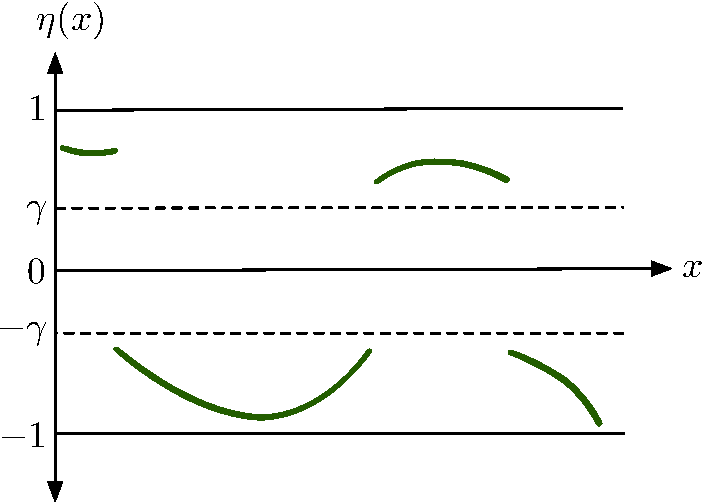
\includegraphics[width=3in]{oned-massart.pdf}
\end{center}
\caption{In this example the conditional probability function $\eta$ is defined by four intervals; on each, $\eta$ is either $> \gamma$ or $<-\gamma$.}
\label{fig:oned-massart}
\end{figure}

We will take $\B$ to consist of all open intervals of $[0,1]$, with $\B(x)$ denoting intervals that contain point $x$. It can be shown that for any $x \in I_j$,
\begin{itemize}
\item $L_1(x) \leq \lg (n/n_j)$, where $n_j = |X \cap I_j|$, and
\item $L_2(x) \leq \lg (n/r(x))$, where $r(x)$ is the minimum number of data points that lie between $x$ and a boundary point ($\lambda_{j-1}$ or $\lambda_j$), counting $x$ as well.
\end{itemize}
A simple counting argument then shows $|\Delta_\ell| \leq (p-1)n/2^{\ell-2}$; that is, the boundary sets shrink in size exponentially. With $L_1$, $L_2$, and $|\Delta_\ell|$ values in place, Theorem~\ref{thm:label-complexity} can be applied directly to give the following label complexity bound.

\begin{thm}
Pick any $0 < \epsilon, \delta < 1$. Suppose we run the algorithm of Figure~\ref{alg:main} with $k = O((1/\gamma^2) \ln (n/\delta))$. With probability at least $1-\delta$, after making
$$ O \left( \frac{p-1}{\gamma^2} \ln \frac{p-1}{\epsilon} \ln \frac{n}{\delta} \right) $$
queries, the algorithm will assign the correct label $g^*(x)$ to at least $1-\epsilon$ fraction of $X$, except possibly the $2k$ points of either side of each boundary point.
\label{thm:oned-massart}
\end{thm}

The $2k$ points nearest each boundary cannot be labeled by our algorithm with any certainty because they lie in intervals with a strongly positive bias as well as in intervals with a strongly negative bias. This qualification would be removed if were allowed to make multiple queries to each point, because in that case we would include $O(k)$ copies of each point, as explained earlier.

\subsection{Example: One-dimensional data with monotonic $\eta$}

We now turn to another one-dimensional setting. Once again, $X$ consists of $n$ arbitrarily-placed points in $\X = [0,1]$. This time, however, they are labeled according to a conditional probability function $\eta: \X \to [-1,1]$ that is continuous and strictly increasing. Let $\lambda \in (0,1)$ denote the point for which $\eta(\lambda) = 0$. Also, let $\lambda_L, \lambda_R$ be the points for which $\eta(\lambda_L) = -\gamma$ and $\eta(\lambda_R) = \gamma$. Thus we are not required to label points in the interval $(\lambda_L, \lambda_R)$. See Figure~\ref{fig:oned-monotonic} for an example.

\begin{figure}
\begin{center}
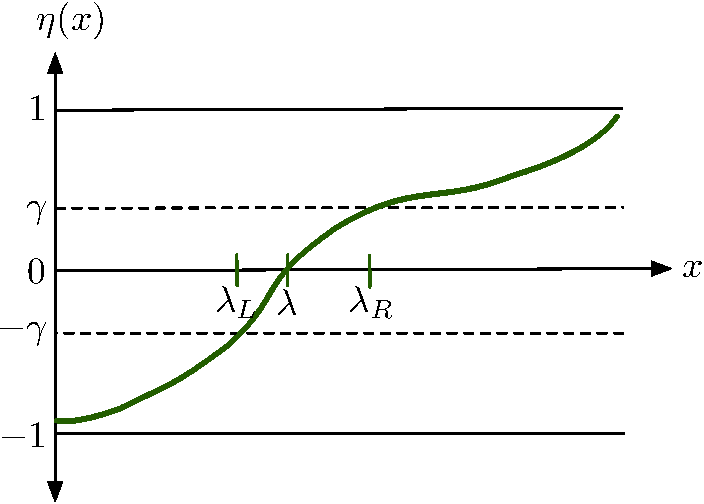
\includegraphics[width=3in]{oned-monotonic.pdf}
\end{center}
\caption{The conditional probability function $\eta$ is monotonically increasing. The values $x = \lambda_L, \lambda, \lambda_R$ have $\eta(x) = -\gamma, 0, \gamma$ respectively.}
\label{fig:oned-monotonic}
\end{figure}


Take $\B$ to consist of all closed intervals, and $\B(x)$ to be intervals containing $x$. It can be shown that for $n^- = |[0,\lambda_L] \cap X|$ and $n^+ = |[\lambda_R,1] \cap X|$, 
\begin{itemize}
\item $L_1(x) \leq \lg (n/n^+)$ if $x \geq \lambda_R$ and $L_1(x) \leq \lg (n/n^-)$ if $x \leq \lambda_L$, and
\item $L_2(x) \leq \lg (n/r(x))$, where $r(x)$ is the number of data points between $x$ and $\lambda$, counting $x$ as well.
\end{itemize}
The boundary region is again exponentially shrinking, $|\Delta_\ell| \leq 4n/2^\ell$, giving the following label complexity bound.


\begin{thm}
Define
\begin{align*}
r^+ &= \min \{r(x): x \in X \cap [\lambda_R,1]\} \\
r^- &= \min \{r(x): x \in X \cap [0,\lambda_L]\} \\
\end{align*}
Pick any $0 < \delta < 1$. Suppose we run the algorithm of Figure~\ref{alg:main} with $k = O((\log n)/\gamma^2)$.  Take any 
$$ m \geq 64k \cdot \max \left( \frac{n}{\min(n^+,n^-)}, \ 2 \lg \frac{\min(n^+,n^-)}{\min(r^+,r^-)} \right) .$$
With probability at least $1-\delta$, after making $m$ queries, the algorithm will correctly label all points $x \in X$ with $|\eta(x)| \geq \gamma$ and $r(x) \geq 2k$.
\label{thm:oned-monotonic}
\end{thm}

For $n^+, n^-, r^+, r^- = \Theta(n)$, this yields a label complexity of $O(\log n)$.

\section{Analysis of algorithm: distributional setting}

We now turn to a setting where the points $X$ are sampled from a distribution $\mu$ on $\X \subset \R^d$. The algorithm is unchanged, but we seek to bound label complexity in terms of properties of $\mu$ and $\eta$.

For simplicity, we will focus on the case where $\mu$ is absolutely continuous with respect to the Lebesgue measure on $\R^d$ and thus admits a density. We will take $\B$ to consist of all open balls $B(x,r) = \{z: \|z-x\| < r\}$, with $\B(x)$ being balls that contain $x$.

\subsection{A generic bound based on a probabilistic notion of distance}

A key quantity in our analysis is a notion of distance based on the probability distribution $\mu$. We take the distance from a point $x$ to a set $S$ to be the probability mass of the smallest ball that contains $x$ and touches $S$.
\begin{defn}
For any $x \in \X$ and $S \subset \X$, define
$$ \dist(x,S) = \inf \{\mu(B): B \in \B(x), B \cap S \neq \emptyset\} .$$ 
\label{defn:prob-dist}
\end{defn}
We will see that $L_2(x)$ can be bounded in terms of such distances. In what follows, for $s \in \{-1,0,+1\}$, take $\X^s$ to denote $\{x \in \X: \sign(\eta(x)) = s\}$.
\begin{lemma}
For any $x \in \X$ with $\eta(x) \neq 0$, let $s(x) = \sign(\eta(x))$. Then
$$ L_2(x) \leq \left\lceil \lg \frac{1}{\dist(x, \X^{-s(x)})} \right\rceil + 1.$$
\label{lemma:L2-bound}
\end{lemma}

We will also use this probabilistic distance to define notions of boundary. We take the $p$-boundary to consist of points that are at distance $\leq p$ from points of the opposite label.
\begin{defn}
For any $p > 0$, define $\partial_p = \{x \in \X: \dist(x, \X^{-s(x)}) \leq p\}$.
\label{defn:boundary}
\end{defn}
Notice that this includes all $x$ with $\eta(x) = 0$.

The $(p,q)$ second-order boundary consists of points at distance $\leq q$ from the $p$-boundary.
\begin{defn}
For any $p,q > 0$, define $\partial_{p,q} = \{x \in \X: \dist(x, \partial_p) \leq q\}$.
\label{defn:boundary2}
\end{defn}

We can bound $\Delta_\ell$, the query region at level $\ell$, in terms of the second-order boundary.
\begin{lemma}
For any $\ell \geq 0$, we have $\Delta_\ell \subset \partial_{4/2^\ell, 2/2^\ell}$.
\label{lemma:delta-continuous}
\end{lemma}

Theorem~\ref{thm:label-complexity} now takes on the following form. 
\begin{thm}
Suppose the active learning algorithm is allowed to make $0 < m \leq n$ queries. Define
$$ \ell_1 = \left\lfloor \lg \frac{m}{32k} \right\rfloor .$$
and let $\ell_2$ be the largest integer $\leq \lg (n/2k)$ such that
$$ \sum_{\ell = \ell_1 + 1}^{\ell_2} 2^\ell \mu(\partial_{4/2^\ell, 2/2^\ell}) \ \leq \ \frac{m}{32k} .$$
Then any point $x \in X$ with $L_1(x) \leq \ell_1$ and $L_2(x) \leq \ell_2$ will have a final label $\yh(x)$ that is correctly set to $g^*(x)$.
\label{thm:label-complexity-dist}
\end{thm}



\subsection{Bounds under two assumptions}

In order to apply Theorem~\ref{thm:label-complexity-dist}, we need to be able to bound two quantities: the levels $L_1(x)$ and $L_2(x)$; and the probability masses of boundary sets $\partial_{p,q}$. To do this, we now introduce two simplifying assumptions.

 Let $\X_\gamma = \{x \in \X: |\eta(x)| \geq \gamma\}$; thus $X \cap \X_\gamma$ is the set of points on which our labels will be judged. We will further divide this set by label: for $s \in \{-1,+1\}$, let $\X^s_\gamma = \{x \in \X: s \cdot \eta(x) \geq \gamma\}$. 
\begin{enumerate}
\item[(A1)] There is an absolute constant $p_o > 0$ for which the following holds: for any $x \in \X_\gamma$, there exists $B \in \B(x)$ such that $B \subset \X^{s(x)}_\gamma$ and $\mu(B) \geq p_o$.
\end{enumerate}
As we will see, this assumption holds if the decision regions have bounded curvature. It allows us to bound $L_1(x)$ easily.
\begin{lemma}
Under (A1), every $x \in \X_\gamma$ has $L_1(x) \leq \lceil \lg (1/p_o) \rceil$.
\label{lemma:L1-bound}
\end{lemma} 
The second assumption is a variant of the Tsybakov margin condition.
\begin{enumerate}
\item[(A2)] There are absolute constants $C > 0$ and $0 < \sigma < 1$ for which the following holds: for any $p > 0$, we have $\mu(\partial_{p,p}) \leq C p^\sigma$.
\end{enumerate}
If, for instance, $\mu$ were the uniform distribution over $[0,1]^d$, we would expect $\sigma \sim 1/d$.

Under (A1) and (A2), we can give concrete label complexity bounds.
\begin{thm}
Assume (A1) and (A2). There is an absolute constant $C'$ for which the following holds. Pick $0 < \delta < 1$ and take $k = O((d \log n)/\gamma^2)$. If the algorithm of Figure~\ref{alg:main} is allowed to make $m \geq 128k/p_o$ queries and $n = \Omega(m^{1/(1-\sigma)})$, then with probability at least $1-\delta$, it will correctly label all but
$$ C' \left(\frac{k}{m}\right)^{\sigma/(1-\sigma)} $$
fraction of $X$.
\label{thm:label-complexity-specific}
\end{thm}

\begin{figure}
\begin{center}
\includegraphics[width=4.5in]{Figures/Focus_sets.pdf}
\end{center}
\caption{A 2D example of the operation of the algorithm.{\bf (a)} A 400x400 square is partitioned in two, one with bias $\eta=0.3$ and the other with bias $\eta=-0.3$. There is a smooth and bounded curvature boundary between the two parts. In addition there is a ball of radius 15 {\bf (c)} with an opposite polarity than it's surroundings. The right hand side {\bf(b)} depicts the focused sampling sets for diferent radii. Note how the focus set becomes increasingly closer to the smooth boundary. Note also that the ball {\bf (c)} does not impact the focus set until $r=10$. This is the case where the prediction for large radii is wrong and is corrected by a ``mind change''}
\label{fig:twod-focus-sets}
\end{figure}

\subsection{Realizing the assumptions}

\yoav{How about the following simplication: keep (C1,C4(simplified)) and replace (C2,C3) by the assumption that $|\eta(x)|>\gamma$ for all $x$, i.e. a jump in the conditional probability at the boundary? }

We'll now see how (A1) and (A2) are consequences of somewhat more commonplace assumptions on data distributions. The first three are standard in nonparametric estimation while the fourth is common in computational geometry.
\begin{enumerate}
\item[(C1)] [Strong density condition] Distribution $\mu$ on $\X \subset \R^d$ admits a density that is bounded below and above: there exist constants $c_o, c > 0$ such that for all balls $B \in \B$,
$$ c_o \vol(B) \leq \mu(B) \leq c \vol(B) ,$$
where $\vol(\cdot)$ is $d$-dimensional volume.
\item[(C2)] [Holder-smoothness of conditional probability function] There exist constants $L, \alpha$ such that
$$ |\eta(x) - \eta(x')| \ \leq \ L \|x - x'\|^\alpha$$
for all $x,x' \in \X$.
\item[(C3)] [Tsybakov margin condition] There exists constants $M, \beta$ such that
$$ \mu(\{x \in \X: |\eta(x)| \leq \tau\}) \leq M \tau^\beta$$
for all $\tau \in (0,1)$.
\item[(C4)] [Bounded curvature] The boundaries $\{x \in \X: \eta(x) = \gamma\}$ and $\{x \in \X: \eta(x) = -\gamma\}$ are manifolds of reach $r_o > 0$.
\end{enumerate}

\begin{lemma}
Conditions (C1) and (C4) yield assumption (A1), with $p_o = r_o^d \cdot c_o \cdot v_d$, where $v_d$ is the volume of the unit ball in $\R^d$.
\label{lemma:A1}
\end{lemma}

\begin{proof}
Pick any $x \in \X_\gamma^+$ (the negative case is similar), and let $r = \inf_{z \in (\X \setminus \X_\gamma^+)}$. If $r \geq r_o$, then $B = B(x,r_o)$ is entirely in $\X_\gamma^+$. Otherwise, the reach condition (C2) implies the existence of a ball $B \subset \X_\gamma^+$ that contains $x$ and has radius $r_o$. Either way, $\mu(B) \geq c_o \vol(B) = c_o v_d r_o^d$ by (C1). 
\end{proof}

\begin{lemma}
Conditions (C1), (C2), and (C3) yield assumption (A2) with $\sigma = \alpha \beta/d$. 
\end{lemma}

\begin{proof}
Under (C1), any ball of probability mass $\leq p$ has volume $\leq p/c_o$ and radius $\leq (p/(c_o v_d))^{1/d}$. Let's call this latter quantity $r$. Thus, any point in $\partial_p$ lies within distance $2r$ of the boundary, while a point in $\partial_{p,p}$ lies within distance $4r$. By (C2), any point in $\partial_{p,p}$ has $|\eta(x)| \leq L (4r)^\alpha$. The total probability mass of such points can then be bounded using (C3):
$$ \mu(\partial_{p,p}) \ \leq \ M (L (4r)^\alpha)^\beta \ = \ M \cdot L^\beta \cdot 4^{\alpha\beta} \cdot \left( \frac{p}{c_o v_d} \right)^{\alpha\beta/d} .$$
\end{proof}

\bibliography{refs}
\bibliographystyle{plain}

\pagebreak
\appendix

\section{Technicalities: discrete setting}

\subsection{Large deviation bounds for the discrete setting}

\begin{lemma}
Fix a confidence parameter $0 < \delta < 1$ and a positive integer $k \geq 6 \ln (4/\delta)$. 

Let $x_1, \ldots, x_m$ be any collection of points. Suppose that the labels $Y_i \in \{-1,1\}$ of these points are independent, with $\E Y_i = \eta(x_i)$. Define
$$ \eta_o = \frac{1}{m} \left( \eta(x_1) + \cdots + \eta(x_m) \right) .$$
Now consider the following estimator $Z$ of this quantity:
\begin{itemize}
\item Each $x_i$ is chosen with probability $q > 0$, independently. Let $N$ be the number of selected points.
\item If $N > 0$, the labels $Y_i$ of the selected points are obtained, and $Z$ is their average.
\end{itemize}
If $qm \geq k + \sqrt{6k \ln (4/\delta)}$, with probability at least $1-\delta$, 
\begin{enumerate}
\item[(a)] $N \geq k$, and 
\item[(b)] $| Z - \eta_o| < \sqrt{(48/k) \ln (4/\delta)}$.
\end{enumerate}
\label{lemma:large-deviation-discrete}
\end{lemma}
\begin{proof}
Let's start with (a). Define $c = \sqrt{3 \ln (4/\delta)}$. We'll take $qm = k + \sqrt{6k \ln (4/\delta)} = k + c \sqrt{2k}$ since this is the worst case. By assumption, $k \geq 2c^2$ and thus $qm \leq 2k$.

Now, $N$ has a binomial($m,q$) distribution. By a multiplicative Chernoff bound, for $0 < \epsilon < 1$, we have
\begin{align*}
\pr(N \geq qm(1+\epsilon)) &\leq e^{-qm\epsilon^2/3} \\
\pr(N \leq qm(1-\epsilon)) &\leq e^{-qm\epsilon^2/2}
\end{align*}
Take $\epsilon = c/\sqrt{qm}$; by the lower bound on $k$, we have $\epsilon \leq 1/2$. Recalling the choice of $c$, we see that with probability at least $1-\delta/2$, we get 
$$(1-\epsilon) qm < N < (1+\epsilon) qm .$$
The lower bound implies $N > qm(1-\epsilon) = qm - c\sqrt{qm} = k + c \sqrt{2k} - c \sqrt{qm} \geq k$.

For (b), define $c, \ldots, C_m \in \{0,1\}$ as random variables indicating whether the corresponding points were selected; that is, $C_i = {\bf 1}(\mbox{$x_i$ was selected})$. The sum of the obtained labels is then $S = c Y_1 + \cdots + C_m Y_m$. Notice that these $C_iY_i \in \{-1,0,1\}$ are independent with $\E[C_iY_i] = q \eta(x_i)$ and $\E[(C_iY_i)^2] = \E[C_i] = q$. Thus their sum $S$ has expectation
$$ \E [S] = \sum_{i=1}^m \E[C_i Y_i] = \sum_{i=1}^m q \eta(x_i) = qm \eta_o $$
and variance
$$ \mbox{var}(S) = \sum_{i=1}^m \mbox{var}(C_iY_i) \leq qm .$$
We can bound the concentration of $S$ around its expected value using Bernstein's inequality, by which
$$ \pr(|S - \E[S]| \geq t) \leq 2 \exp \left( - \frac{t^2}{2(\mbox{var}(S) + t/3)} \right) .$$
Using $t = \epsilon qm$, we then have that $|S - qm \eta_o| \leq \epsilon qm$ with probability at least $1-\delta/2$.

Combining with the high-probability bound on $N$ above, we get
$$ \frac{qm \eta_o - \epsilon qm}{qm(1+\epsilon)} < \frac{S}{N} < \frac{qm \eta_o + \epsilon qm}{qm(1-\epsilon)},$$
whereupon (recalling $Z = S/N$)
$$ 
\eta_o \left( \frac{1}{1+\epsilon} -1 \right) - \frac{\epsilon}{1+\epsilon} < Z - \eta_o < \eta_o \left( \frac{1}{1-\epsilon} - 1 \right) + \frac{\epsilon}{1-\epsilon} .$$
Since $|\eta_o| \leq 1$,
$$ |Z - \eta_o | < \max \left( \frac{2\epsilon}{1+\epsilon}, \frac{2\epsilon}{1-\epsilon} \right)
\leq 
4 \epsilon,$$
as claimed.  
\end{proof}

\subsection{Large deviation bounds for the continuous setting}

Let $\mu$ be a distribution on the instance space $\X$.

\begin{lemma}[checked]
Fix a confidence parameter $0 < \delta < 1$ and a positive integer $k \geq 6 \ln (4/\delta)$. 

Pick a set $B \subset \X$ with $\mu(B) > 0$. Suppose $m$ points $x_1, \ldots, x_m$ are drawn from $\mu|_B$, the restriction of $\mu$ to $B$, and their labels $y_1, \ldots, y_m \in \{-1,+1\}$ are generated according to $\eta$, that is, $\E[Y_i|x_i] = \eta(x_i)$.

Consider the following estimator $Z$ of $\eta(B)$:
\begin{itemize}
\item Each $x_i$ is chosen with probability $q > 0$, independently. Let $N$ be the number of selected points.
\item The labels of the selected points are averaged, yielding a value $Z$ (which defaults to 0 if no points were selected).
\end{itemize}
If $qm \geq k + \sqrt{6k \ln (4/\delta)}$, with probability at least $1-\delta$, 
\begin{enumerate}
\item[(a)] $N \geq k$, and 
\item[(b)] $| Z - \eta(B)| < \sqrt{(48/k) \ln (4/\delta)}$.
\end{enumerate}
\label{lemma:large-deviation-continuous}
\end{lemma}

\begin{proof}
This exactly follows the proof of Lemma~\ref{lemma:large-deviation-discrete}, with $\eta(B)$ in place of $\eta_o$.
\end{proof}

Next, we show that the $\eta_X(B)$ are, in turn, close to the corresponding $\eta(B)$.
\begin{lemma}
Fix any confidence parameter $0 < \delta < 1$. Then with probability at least $1-\delta$, the following holds for all $B \in \B$:
$$ \left| \eta(B) - \eta_X(B) \right| \leq \sqrt{\frac{2}{|X_B|} \ln \frac{2|\B|}{\delta}} .$$
\label{lemma:discrete-to-continuous}
\end{lemma}
\begin{proof}
Pick any $B \in \B$. The points in $X_B$ are random draws from $\mu|_B$. Each such point $Z$ has $\eta(Z) \in [-1,1]$ with $\E[\eta(Z)] = \eta(B)$. By a Hoeffding bound,
$$ \pr(|\eta_X(B) - \eta(B)| \geq t) \leq 2e^{-t^2|X_B|/2} $$
for any $t > 0$. The result follows by taking 
$$t = \sqrt{\frac{2}{|X_B|} \ln \frac{2|\B|}{\delta}}$$ 
and applying a union bound over all $B \in \B$.
\end{proof}

\subsection{Proof of Lemma~\ref{lemma:accurate-bias-estimates}}

We will use Lemma~\ref{lemma:large-deviation-discrete} to obtain a uniform guarantee on the bias estimates for all balls $B \in \B$.

Recall that each point $x \in X$ gets a label $Y \in \{-1,+1\}$ according to the distribution
$$ \eta(x) = \E[y | x].$$ 
For any $B \in \B$ with $X_B \neq \emptyset$, let $\eta_X(B)$ be the average $\eta$-value of the points in $B$, that is,
$$ \eta_X(B) = \frac{1}{|X_B|} \sum_{x \in X_B} \eta(x) .$$

Recall the definitions of the constant $c$ from (\ref{eq:c1}) and that for each level $\ell$:
\begin{equation}
\tau_\ell = \min \left( \frac{2^{\ell+2}k}{n}, \ 1 \right)
\label{eq:threshold-ell}
\end{equation}


. For any $B \in \B_\ell$, define its \emph{query-set} to be $\Gamma(B) = \{z \in X_B: T_z \leq \tau_\ell\}$. We base our bias-estimate for $B$ on the labels of points in $\Gamma(B)$.

\begin{lemma}
Suppose $k \geq 2c^2$. With probability at least $1-\delta$, the following is true for all $B \in \B$ with $|X_B| \geq k$:
\begin{enumerate}
\item[(a)] The query set $\Gamma(B)$ has size at least $k$.
\item[(b)] The average label on $\Gamma(B)$, call it $\widehat{\eta}(B)$, satisfies
$$ \left| \widehat{\eta}(B) - \eta_X(B) \right| \leq \frac{4c}{\sqrt{k}}.$$
\end{enumerate}
\label{lemma:large-deviation-bounds}
\end{lemma}
\begin{proof}
These follow immediately by applying Lemma~\ref{lemma:large-deviation-discrete} to each $B \in \B$ and taking a union bound. In particular, note that the choice of $\tau_\ell$ ensures $|X_B| \tau_\ell \geq 2k$.
\end{proof}

The following corollary of Lemma~\ref{lemma:large-deviation-bounds} is immediate.
\begin{cor}
Suppose that $k \geq (8c/\gamma)^2$. For each $B \in \B$, let $\widehat{\eta}(B)$ be the average label on the query-set $\Gamma(B)$, and define the bias-estimate $\yh(B)$ as follows:
$$ \yh(B)
= 
\left\{
\begin{array}{ll}
\sign(\widehat{\eta}(B)) & \mbox{if $|\widehat{\eta}(B)| \geq \gamma/2$} \\
0 & \mbox{otherwise}
\end{array}
\right.
$$
With probability $\geq 1-\delta$, all bias estimates $\yh(B)$, for $B \in \B$, are $\gamma$-accurate.
\label{cor:accurate-bias-estimates}
\end{cor}
\begin{proof}
By the choice of $k$, we have from Lemma~\ref{lemma:large-deviation-bounds} that 
$| \widehat{\eta}(B) - \eta_X(B) | < \gamma/2$
for all $B \in \B$.
\end{proof}

\subsection{Proof of Lemma~\ref{lemma:boundary}}

For part (a), note that some $B_o \in \B_{L_1(x)}(x)$ has significant bias towards the correct label $s(x)$, as does any ball $B \in \B(x)$ contained within it. For $\ell \geq L_1(x)$, the set $\{B \in \B_{\leq \ell(x)}: X_{B} \subseteq X_{B_o}\}$ is nonempty (it contains $B_o$); pick any minimal ball $B$ within it. Then $\yh(B) = s(x)$ and thus $s(x) \in \PL_\ell(x)$.

For (b), take any $\ell \geq L_2(x)$. Consider any $B \in \B_{\leq \ell}(x)$ for which $s(x) \cdot \eta_X(B) < -b_1$. By definition of $L_2(x)$, this $B$ must lie in $B_{< L_2(x)}(x)$, and moreover there must exist $B' \in \B_{\leq L_2(x)}(x) \subset \B_{\leq \ell}(x)$ with $X_{B'} \subset X_B$ and $s(x) \cdot \eta_X(B') \geq -b_1$. Thus, any minimal $B \in \B_{\leq \ell}(x)$ has $\yh(B) \in \{0, s(x)\}$; whereupon $-s(x) \not\in \PL_\ell(x)$.

\subsection{Proof of Lemma~\ref{lemma:focused}}

Let $\overline{U}_\ell$ denote the set of all points that are ever (in any round of sampling) in the uncertainty set at level $\ell$. From Lemma~\ref{lemma:boundary}(b), we see that any $x$ with $L_2(x) < \ell$ has $\yh_{\ell-1}(x) \neq \ !$ and thus never makes it into the uncertainty set at level $\ell$. In short,
\begin{equation}
\overline{U}_{\ell} \subset \{x \in X: L_2(x) \geq \ell\}.
\label{eq:uncertainty}
\end{equation}

We see from the {\tt Focused-query} subroutine (Figure~\ref{alg:sampling}) that all focused samples at level $\ell$ lie in
$$
\bigcup_{x \in \overline{U}_\ell} \bigcup_{B \in \B_\ell(x)} \{z \in X_B: T_z \leq \tau_\ell \}
\ 
\subset 
\ 
\bigcup_{x \in X: L_2(x) \geq \ell} \bigcup_{B \in \B_\ell(x)} \{z \in X_B: T_z \leq \tau_\ell \}
\ 
=
\ 
\{z \in \Delta_\ell: T_z \leq \tau_\ell \}.
$$

\subsection{Proof of Theorem~\ref{thm:label-complexity}}

We start by showing that various subsets of interest contain roughly the expected number of points at each level.
\begin{lemma}
Pick any $0 < \ell_o \leq \lg (n/2k)$. With probability at least $1-2(\ell_o+1)e^{-k/3}$, the following hold for all levels $0 \leq \ell \leq \ell_o$.
\begin{enumerate}
\item[(a)] $|\{x \in X: T_x \leq \tau_\ell\}| < 2 n \tau_\ell$.
\item[(b)] If $\Delta_\ell \neq \emptyset$ then $|\{x \in \Delta_{\ell}: T_x \leq \tau_\ell\}| < 2 |\Delta_\ell| \tau_\ell$.
\end{enumerate}
\label{lemma:level-distribution}
\end{lemma}
\begin{proof} 
Pick any subset $S \subset X$ and let $m = |S|$. Then $|\{x \in S: T_x \leq \tau_\ell\}|$ has a $\mbox{binomial}(m, \tau_\ell)$ distribution with expectation $m \tau_\ell$. The probability that it is greater than or equal to twice its expected value is, by a multiplicative Chernoff bound, at most $e^{-m \tau_{\ell}/3}$, which is $\leq e^{-k/3}$ as long as $m \tau_\ell \geq k$.

Both parts follow from this principle; and we take a union bound over all $\ell_o + 1$ levels. For (b), we need to check that $|\Delta_\ell| \tau_\ell \geq k$. To see this, observe from the definition (\ref{eq:sampling-region}) of $\Delta_\ell$ that if it is non-empty, then it contains $X_B$ for at least one ball $B \in \B_\ell$, and every such ball has at least $n/2^{\ell+1}$ points. Combining this with the definition (\ref{eq:threshold-ell}) of $\tau_\ell$ yields $|\Delta_\ell| \tau_\ell \geq k$.
\end{proof}

We now begin on the proof of Theorem~\ref{thm:label-complexity}.

Denote the first $m/2$ queries by {\it phase one} and the second $m/2$ by {\it phase two}. We will analyze the effect of background sampling in phase one and focused sampling in phase two. We start with the former.

Of the $m/2$ queries in phase one, at least $m/4$ will be background samples. Therefore the $m/4$ points with lowest $T_x$ values are guaranteed to be queried.

Now, for $\ell_1$ as defined, we have from (\ref{eq:threshold-ell}) that $\tau_{\ell_1} \leq m/8n$ and thus from Lemma~\ref{lemma:level-distribution}(a) that at most $m/4$ points in $X$ satisfy $T_x \leq \tau_{\ell_1}$. Therefore all such points are queried in phase one, and all label-estimates $\{\yh_{\ell_1}(x): x \in X\}$ are set.

It then follows from Lemma~\ref{lemma:boundary}(a) that the following hold for any $x \in X$ with $L_1(x) \leq \ell_1$:
\begin{enumerate}
\item[(a)] By the end of phase one, $\yh_{\ell_1}(x) \in \{g^*(x), !\}$.
\item[(b)] For any $\ell > \ell_1$, when $\yh_\ell(x)$ becomes available, it lies in $\{g^*(x), !\}$.
\item[(c)] If $x$ ever leaves the combined uncertainty region $U = \cup_\ell U_\ell$ during phase two, then its final label as defined in (\ref{eq:final-label}) is henceforth always $\yh(x) = g^*(x)$.
\end{enumerate}

Now let's move on to phase two. Let $A = \{x \in X: L_1(x) \leq \ell_1, L_2(x) \leq \ell_2\}$. We will show that every point in $A$ must leave the uncertainty region $U$ at some time during phase two. From (c), we can conclude that all these points have their final labels set correctly, once and for all.

We will break the argument into two cases. 

{\it Case 1:} Fewer than $m/4$ focused queries are made in phase two. This can only happen if some round of sampling has an empty uncertainty set, meaning that all of $A$ has left $U$ at that point.

{\it Case 2:} A full $m/4$ focused queries are made in phase two. By the analysis of phase one, none of these queries can be at level $\leq \ell_1$ and by Lemma~\ref{lemma:focused}, the total number of possible focused queries at levels $\ell_1+1$ through $\ell_2$ inclusive is at most
$$\sum_{\ell=\ell_1+1}^{\ell_2} |\{z \in \Delta_{\ell}: T_z \leq \tau_\ell \}| 
\ < \ 
\sum_{\ell=\ell_1+1}^{\ell_2} 2 |\Delta_{\ell}| \tau_\ell
\ \leq \ 
\frac{m}{4} ,
$$
where the first inequality is from Lemma~\ref{lemma:level-distribution}(b). Thus at least one query in phase two must be at level $\ell_2 +1$. When this query is made, every $U_\ell$ with $\ell \leq \ell_2$ must be empty and thus all of $A$ must have left the uncertainty region; recall from (\ref{eq:uncertainty}) that no $x \in A$ can be part of $U_\ell$ for $\ell > \ell_2 \geq L_2(x)$. 

Thus every $x \in A$ must leave the uncertainty region at some point in phase two, and their final labels are subsequently set correctly.

\subsection{Proof of Theorem~\ref{thm:oned-massart}}

We begin with bounds on the $L_1$ and $L_2$ levels for each point.
\begin{lemma}
Pick any $x \in \X$; suppose $x \in I_j$.
\begin{enumerate}
\item[(a)] Let $n_j = |X \cap I_j|$. Then $L_1(x) \leq \lg (n/n_j)$.
\item[(b)] Let $r(x)$ be the minimum number of data points that lie between $x$ and a boundary point, counting $x$ as well; this is either the number of points in the left-interval $(\lambda_{j-1},x]$ (if $j > 1$) or the right-interval $[x, \lambda_j)$ (if $j < p$), whichever is smaller. Then $L_2(x) \leq \lg (n/r(x))$.
\end{enumerate}
\label{lemma:oned-massart-L}
\end{lemma}
\begin{proof}
For (a), notice first that $I_j \in \B_{\ell}(x)$ for $\ell = \lceil (\lg n/n_j) - 1 \rceil$. Moreover, $s(I_j) \cdot \eta_X(I_j) > \gamma \geq b_2$. Thus $I_j$ belongs to $\B_\ell(x)$ and is strongly biased towards the correct label. This strong bias also holds for any subset of $I_j$. 

For (b), consider any $\ell \geq \lg (n/r(x))$. Any $B \in \B(x)$ with $\mbox{sign}(\eta_X(B)) \neq s(I_j)$ must contain either the entire left-interval $(\lambda_{j-1},x]$ or the entire right-interval $[x, \lambda_j)$, and thus has at least $r(x)$ points, which means that it is too large to be in $\B_\ell$. Thus all intervals $B \in \B_{\geq \ell}(x)$ have $s(I_j) \cdot \eta_X(B) > 0$. Also, for any interval $B \in \B_{<\ell}(x)$ there is some $B' \in \B_{\ell}(x)$ that is strictly contained within it.
\end{proof}

With $L_1(x)$ and $L_2(x)$ under control, it is easy to bound the size of the focused query region $\Delta_\ell$ at each level.
\begin{lemma}
For any $\ell \geq 0$, let $\Delta_\ell$ denote the focused querying region at level $\ell$, as defined in (\ref{eq:sampling-region}). Then $|\Delta_\ell| \leq (p-1)n/2^{\ell-2}$.
\label{lemma:oned-massart-query-region}
\end{lemma}

\begin{proof}
We have
\begin{align*}
\Delta_\ell 
&= \bigcup_{x \in X: L_2(x) \geq \ell} \bigcup_{B \in \B_{\ell}(x)} (B \cap X) \\
&\subset \bigcup_{x \in X: r(x) \leq n/2^\ell} \bigcup_{B \ni x: |B \cap X| < n/2^\ell} (B \cap X) 
.
\end{align*}
This includes at most $n/2^{\ell-1}$ points from $X$ on either side of each boundary point $\lambda_j$.
\end{proof}

We are now ready to establish Theorem~\ref{thm:oned-massart}.

Setting $k$ to $O((1/\gamma^2) \ln (n/\delta))$ satisfies the requirements of Lemma~\ref{lemma:accurate-bias-estimates}. Here we are using the fact that although $\B$ is infinite, we need only consider $O(n^2)$ distinct intervals since $|X| = n$.

Next, using Lemma~\ref{lemma:oned-massart-query-region}, we have that for any integers $0 \leq \ell_1 < \ell_2$,
$$ \sum_{\ell = \ell_1+1}^{\ell_2} |\Delta_\ell| \tau_\ell
\ \leq \ 
\sum_{\ell = \ell_1+1}^{\ell_2} \frac{(p-1) n}{2^{\ell-2}} \cdot \frac{2^{\ell+2}k}{n}
\ = \ 
16(p-1)k (\ell_2 - \ell_1).
$$
We can then apply Theorem~\ref{thm:label-complexity} to conclude that $m$ query points are enough to correctly classify all $x \in X$ with $L_1(x) \leq \ell_1$ and $L_2(x) \leq \ell_2$, for
\begin{align*}
\ell_1
&= 
\left\lfloor \lg \frac{m}{32k} \right\rfloor \\
\ell_2
&=
\min \left( \ell_1 + \frac{m}{128 k(p-1)}, \ \lg \frac{n}{2k} \right)
\end{align*}
Using Lemma~\ref{lemma:oned-massart-L}, we have that in every target interval $I_j$ with $n_j/n = \Omega(k/m)$, all but $n \cdot 2^{-\ell_2-1}$ points will be correctly classified. For large enough $m$, this means that the fraction of misclassified or unclassified points in $X$ will be at most $\epsilon$ after $O(k(p-1) \log ((p-1)/\epsilon))$ queries, apart from the $2k$ points nearest the boundaries, which will remain unclassified.

\subsection{Proof of Theorem~\ref{thm:oned-monotonic}}

We begin by bounding the critical levels $L_1$ and $L_2$ for points in $X$.
\begin{lemma}
Pick any $x \in [0, 1]$.
\begin{enumerate}
\item[(a)] Define $n^- = |[0,\lambda_L] \cap X|$ and $n^+ = |[\lambda_R,1] \cap X|$. Then
$$
L_1(x)
\leq
\left\{
\begin{array}{ll}
\lg (n/n^+) & \mbox{if $x \geq \lambda_R$} \\
\lg (n/n^-) & \mbox{if $x \leq \lambda_L$}
\end{array}
\right.
$$
\item[(b)] Let $r(x)$ be the number of points between $x$ and the boundary point $\lambda$, counting $x$ itself. That is, $r(x) = |[x,\lambda) \cap X|$ if $x < \lambda$, or $|(\lambda, x] \cap X|$ if $x > \lambda$. Then $L_2(x) \leq \lg (n/r(x))$.
\end{enumerate}
\label{lemma:oned-monotonic-L}
\end{lemma}
\begin{proof}
For (a), take any $x \geq \lambda_R$ (the other case is similar). The interval $B = [\lambda,1]$ lies in $\B_\ell(x)$ for $\ell = \lceil \lg (n/n^+) - 1 \rceil$ and has $\eta_X(B) \geq b_2$. Furthermore, any $B' \subset B$ also has $\eta_X(B') \geq b_2$. 

For (b), take $x \geq \lambda_R$ and $\ell \geq \lg (n/r(x))$. Any $B \in \B_\ell(x)$ contains $< n/2^\ell \leq r(x)$ points and thus cannot possibly extend to the other side of the boundary. It follows that every $B \in \B_{\geq \ell}(x)$ has $\eta_X(B) \geq 0$. Moreover, any interval $B'$ that does extend to the other side of the boundary contains $B' \in \B_{\ell}(x)$ that is entirely on the same side as $x$.
\end{proof}

We can now bound the size of the query region at each level, in much the same way as we did for our previous one-dimensional example.
\begin{lemma}
For any $\ell \geq 0$, let $\Delta_\ell$ denote the focused querying region at level $\ell$, as defined in (\ref{eq:sampling-region}). Then $|\Delta_\ell| \leq 4n/2^\ell$.
\label{lemma:oned-monotonic-query-region}
\end{lemma}

\begin{proof}
The bound on $L_2(x)$ from Lemma~\ref{lemma:oned-monotonic-L} is the same as in our earlier one-dimensional example. We can use the same proof as in Lemma~\ref{lemma:oned-massart-query-region}, with $p=2$, to get the stated bound.
\end{proof}

We are now ready for the proof of Theorem~\ref{thm:oned-monotonic}.

First observe that for any $\ell_1 \leq \ell_2$, we have from Lemma~\ref{lemma:oned-monotonic-query-region} that
$$ \sum_{\ell=\ell_1+1}^{\ell_2} |\Delta_\ell| \tau_\ell 
\ \leq \ \sum_{\ell=\ell_1+1}^{\ell_2} \frac{4n}{2^\ell} \cdot \frac{2^{\ell+2} k}{n} 
\ = \ 16k(\ell_2-\ell_1).$$
Now, let's define
$$ \ell_1 = \left\lfloor \lg \frac{m}{32k} \right\rfloor, 
\ \ \ \ell_2 = \min \left( \ell_1 + \frac{m}{128k}, \ \ \lg \frac{n}{2k} \right).$$
Then for any $x \in [0, \lambda_L] \cup [\lambda_R,1]$, we have
$$ \ell_1 = \left\lfloor \lg \frac{m}{32k} \right\rfloor 
\ \geq \ 
\lg \frac{m}{64k}
\ \geq \ 
\lg \frac{n}{\min(n^+,n^-)}
\ \geq \ 
L_1(x)$$
and, if $\min(r^+, r^-) \geq 2k$,
$$ \ell_2 
\ = \ \ell_1 + \frac{m}{128k} 
\ \geq \ \lg \frac{m}{64k} + \lg \frac{\min(n^+,n^-)}{\min(r^+,r^-)} 
\ \geq \ \lg \frac{m}{64k} + \lg \frac{64kn/m}{\min(r^+,r^-)} 
\ = \ \lg \frac{n}{\min(r^+,r^-)}
\ \geq \ 
L_2(x).
$$
We get the algorithmic guarantee by applying Theorem~\ref{thm:label-complexity}. 

\section{Technicalities: distributional setting}

In the distributional setting, $X$ is drawn i.i.d.\ from a distribution $\mu$ on $\X \subset \R^d$.  We assume $\mu$ is absolutely continuous with respect to the Lebesgue measure on $\R^d$ and thus admits a density. Take $\B$ to consist of all open balls $B(x,r) = \{z: \|z-x\| < r\}$, with $\B(x)$ being balls that contain $x$.

\subsection{Sampling level and probability mass}

To begin with, we relate the number of points in a ball $B \in \B$ (and thus the level of the ball) to its probability mass under the marginal distribution.
\begin{lemma}
With probability at least $1-\delta$, for all $B \in \B$ with $n \mu(B) \geq 12 \ln (2|\B|/\delta)$, we have
$$ \frac{\mu(B)}{2} \leq \frac{|X_B|}{n} \leq 2 \mu(B) .$$
\label{lemma:ball-size-bounds}
\end{lemma}
\begin{proof}
It is an immediate consequence of the multiplicative Chernoff bound that with probability at least $1-\delta$, for all $B \in \B$,
$$ \frac{|X_B|}{n} = \mu(B) \left(1 \pm \sqrt{\frac{3}{n \mu(B)} \ln \frac{2|\B|}{\delta}} \right) .$$
\end{proof}

Henceforth assume that this high-probability event holds. Next, we will see that balls of probability mass $p$ belong to level $\ell \approx \lg (1/p)$.
\begin{lemma}
For any level $\ell \geq 0$ and any $B \in \B_{\ell}$,
$$ \left\lceil \lg \frac{1}{\mu(B)} \right\rceil -2 \leq \ell \leq  \left\lceil \lg \frac{1}{\mu(B)} \right\rceil.$$
\label{lemma:mass-vs-level}
\end{lemma}
\begin{proof}
Recall the definition of level $\ell$:
$$ B \in \B_\ell 
\ \Longleftrightarrow \ \frac{n}{2^{\ell+1}} \leq |X_B| < \frac{n}{2^\ell} 
\ \Longleftrightarrow \ 2^\ell < \frac{n}{|X_B|} \leq 2^{\ell + 1}.$$
By Lemma~\ref{lemma:ball-size-bounds}, 
$$ \frac{1}{2 \mu(B)} \leq \frac{n}{|X_B|} \leq \frac{2}{\mu(B)}.$$
Thus we must have $2^{\ell} < 2/\mu(B)$ and $1/(2 \mu(B)) \leq 2^{\ell+1}$. These translate into the stated bounds on $\ell$.
\end{proof}

\subsection{Proof of Lemma~\ref{lemma:L2-bound}}

Let $p = \dist(x, \X^{-s(x)})$. If $p = 0$, the statement is vacuous, so assume $p > 0$.

Consider $\ell = \lceil \lg (1/p) \rceil + 1$. For any $B \in \B_{\geq \ell}(x)$, we have $\mu(B) \leq 2|X_B|/n < 2/2^\ell \leq p$, using Lemma~\ref{lemma:ball-size-bounds}, the definition of sampling levels, and the definition of $\ell$, in that order. It follows that $B$ does not intersect $\X^{-s(x)}$, whereupon $s(x) \cdot \eta_X(B) \geq 0 \geq -b_1$.

Next, pick any $B \in \B_{\leq \ell}(x)$ with $s(x) \cdot \eta_X(B) < -b_1$. Thus $B$ must intersect $\X^{-s(x)}$. We will show that there exists $B' \in \B_{\leq \ell}(x)$ such that $B' \subset B$ and $B'$ does not intersect $\X^{-s(x)}$; whereupon $s(x) \cdot \eta_X(B') \geq -b_1$. Indeed, take $B' \in \B(x)$ to be a subset of $B$ of mass $p-\epsilon$ for some very small $\epsilon$; we can do this because of the absolute continuity of $\mu$. Then $B'$ does not touch $\X^{-s(x)}$ and by Lemma~\ref{lemma:mass-vs-level}, it lies at level $\leq \ell$.

\subsection{Proof of Lemma~\ref{lemma:delta-continuous}}

Recall from (\ref{eq:sampling-region}) that
$$ \Delta_\ell = \bigcup_{x \in X: L_2(x) \geq \ell} \bigcup_{B \in \B_{\ell}(x)} X_B .$$
Consider any $z \in \Delta_\ell$. Then there exists $x \in \X$ with $L_2(x) \geq \ell$ and $B \in \B_\ell(x)$ such that $z \in B$. Now, $B \in \B_\ell(x)$ implies $|X_B|/n < 1/2^\ell$ and so (by Lemma~\ref{lemma:ball-size-bounds}) $\mu(B) < 2/2^\ell$. We will show that $x \in \partial_{4/2^\ell}$ and thus $z \in \partial_{4/2^\ell, 2/2^{\ell}}$.

Since $L_2(x) \geq \ell$, we have from Lemma~\ref{lemma:L2-bound} that
$$ \ell 
\ \leq \ \left\lceil \lg \frac{1}{\dist(x,\X^{-s(x)})} \right\rceil + 1 
\ \leq \ 
\lg \frac{1}{\dist(x,\X^{-s(x)})} + 2 .
$$
Thus $\dist(x, \X^{-s(x)}) \leq 1/2^{\ell-2}$ and $x \in \partial_{4/2^\ell}$.

\subsection{Proof of Theorem~\ref{thm:label-complexity-dist}}

We will need to relate the size of the query region $\Delta_\ell$ to the probability mass of the corresponding second-order boundary. For this, we provide an analog of Lemma~\ref{lemma:level-distribution} for the distributional setting.
\begin{lemma}
Pick any $0 < \ell_o \leq \lg (n/2k)$. With probability at least $1-2(\ell_o+1)e^{-k/3}$, the following hold for all levels $0 \leq \ell \leq \ell_o$.
\begin{enumerate}
\item[(a)] $|\{x \in X: T_x \leq \tau_\ell\}| \leq 2 n \tau_\ell$.
\item[(b)] $|\{x \in \Delta_{\ell}: T_x \leq \tau_\ell\}| \leq 2 n \mu(\partial_{4/2^\ell, 2/2^\ell}) \tau_\ell$.
\end{enumerate}
\label{lemma:level-distribution-dist}
\end{lemma}
\begin{proof} 
Part (a) is as in Lemma~\ref{lemma:level-distribution}. 

For (b), pick any subset $S \subset \X$. If $X$ consists of $n$ independent draws from $\mu$, then $|\{x \in S: T_x \leq \tau_\ell\}|$ has a $\mbox{binomial}(n, \mu(S) \tau_\ell)$ distribution with expectation $n \mu(S) \tau_\ell$. The probability that it is more than twice its expected value is, by a multiplicative Chernoff bound, at most $e^{-n \mu(S) \tau_\ell/3}$. We will apply this to the various sets $S = \partial_{4/2^\ell, 2/2^\ell}$ and take a union bound over them. In each application, we will also see that $n \mu(S) \tau_\ell \geq k$.

Pick any $\ell \leq \lg (n/2k)$. If $\partial_{4/2^\ell, 2/2^\ell} = \emptyset$, then the statement in (b) is trivially true given Lemma~\ref{lemma:delta-continuous}. So assume this is not the case. Writing $p = 4/2^\ell$, we need to check that $\mu(\partial_{p, p/2}) \tau_\ell \geq k/n$, or equivalently, $\mu(\partial_{p, p/2}) \geq \max(1/2^{\ell+2}, k/n)$. Now, $\partial_{p,p/2} \neq \emptyset \Longrightarrow \partial_p \neq \emptyset$, which means that there exists some ball $B$ of probability mass $<p$ that straddles the decision boundary, in the sense of touching both $\X^+$ and $\X^-$. By absolute continuity of $\mu$, we can grow this ball to probability mass arbitrarily close to $p$ while retaining the boundary-crossing property. Thus $\mu(\partial_p) \geq p$, whereupon $\mu(\partial_{p,p/2}) \geq p$ as well. The required conditions then follow from the value of $p$.
\end{proof}

With this in place, the proof of Theorem~\ref{thm:label-complexity-dist} follows that of Theorem~\ref{thm:label-complexity}; the only change is to use Lemma~\ref{lemma:level-distribution-dist}(b) in place of Lemma~\ref{lemma:level-distribution}(b).

\subsection{Proof of Lemma~\ref{lemma:L1-bound}}

Pick any $x \in X_\gamma$; apply (A1) to get $B \in \B(x)$ for which $\mu(B) \geq p_o$ and $B \subset \X^{s(x)}_\gamma$. By Lemma~\ref{lemma:mass-vs-level}, $B \in \B_\ell$ for $\ell \leq \lceil \lg (1/p_o) \rceil$. Now, $s(x) \cdot \eta_X(B) \geq \gamma$; moreover, for any $B' \in \B(x)$ with $X_{B'} \subset X_B$ we have $X_{B'} \subset \X^{s(x)}_\gamma$ and thus $s(x) \cdot \eta_X(B') \geq \gamma$ as well.

\subsection{Proof of Theorem~\ref{thm:label-complexity-specific}}

In this case, $\B$ is infinite, but by standard VC-dimension arguments there are effectively only $O(n^d)$ distinct balls $B$, in the sense of having different sets $X_B$. This governs the setting of $k$.

First, define $\ell_1 = \lfloor \lg (m/32k) \rfloor$ and observe that by Lemma~\ref{lemma:L1-bound}, all points in $\X_\gamma$ have 
$$ L_1(x) 
\ \leq \ 
\left\lceil \lg \frac{1}{p_o} \right\rceil
\ \leq \ 
\lg \frac{2}{p_o} 
\ \leq \ 
\lg \frac{m}{64k}
\ \leq \ 
\ell_1 .
$$
Next, pick  
$$ \ell_2 = \left\lfloor \frac{1}{1-\sigma} \left( \lg \frac{m}{32k} + \lg \frac{2^{1-\sigma}-1}{C \cdot 2^{1+\sigma}} \right) \right\rfloor.$$
The lower bound on $n$ ensures that this is at most $\lg (n/2k)$. Then,
$$
\sum_{\ell = \ell_1+1}^{\ell_2} 2^\ell \mu(\partial_{4/2^\ell, 2/2^\ell})
\ \leq \ 
C \sum_{\ell = \ell_1+1}^{\ell_2} 2^\ell \left( \frac{4}{2^\ell} \right)^\sigma 
\ \leq \ 
C \cdot 4^\sigma \cdot \frac{2^{1-\sigma}}{2^{1-\sigma}-1} \cdot 2^{(1-\sigma)\ell_2}
\ \leq \ 
\frac{m}{32k} .
$$
Applying Theorem~\ref{thm:label-complexity-dist}, we then see that all points in $\X_\gamma$ with $L_2(x) \leq \ell_2$ will be correctly classified. Any remaining point $x \in \X_\gamma$ has $L_2(x) > \ell_2$ and thus (by Lemma~\ref{lemma:L2-bound})
$$ \left\lceil \lg \frac{1}{\dist(x, \X^{-s(x)})} \right\rceil + 1 > \ell_2 
\ \Longrightarrow \ 
\dist(x, \X^{-s(x)}) < \frac{4}{2^{\ell_2}} \leq C'' \left( \frac{k}{m} \right)^{1/(1-\sigma)} 
$$
for some constant $C''$. Under (A2), which implies the same bound on $\mu(\partial_p)$, the fraction of such points is $\leq C' (k/m)^{\sigma/(1-\sigma)}$ for constant $C'$.

\end{document}

%%% Local Variables:
%%% mode: latex
%%% TeX-master: t
%%% End:
